\section{System design on Apache Kafka}\label{sec:system}

\begin{figure*}[t]
\centering
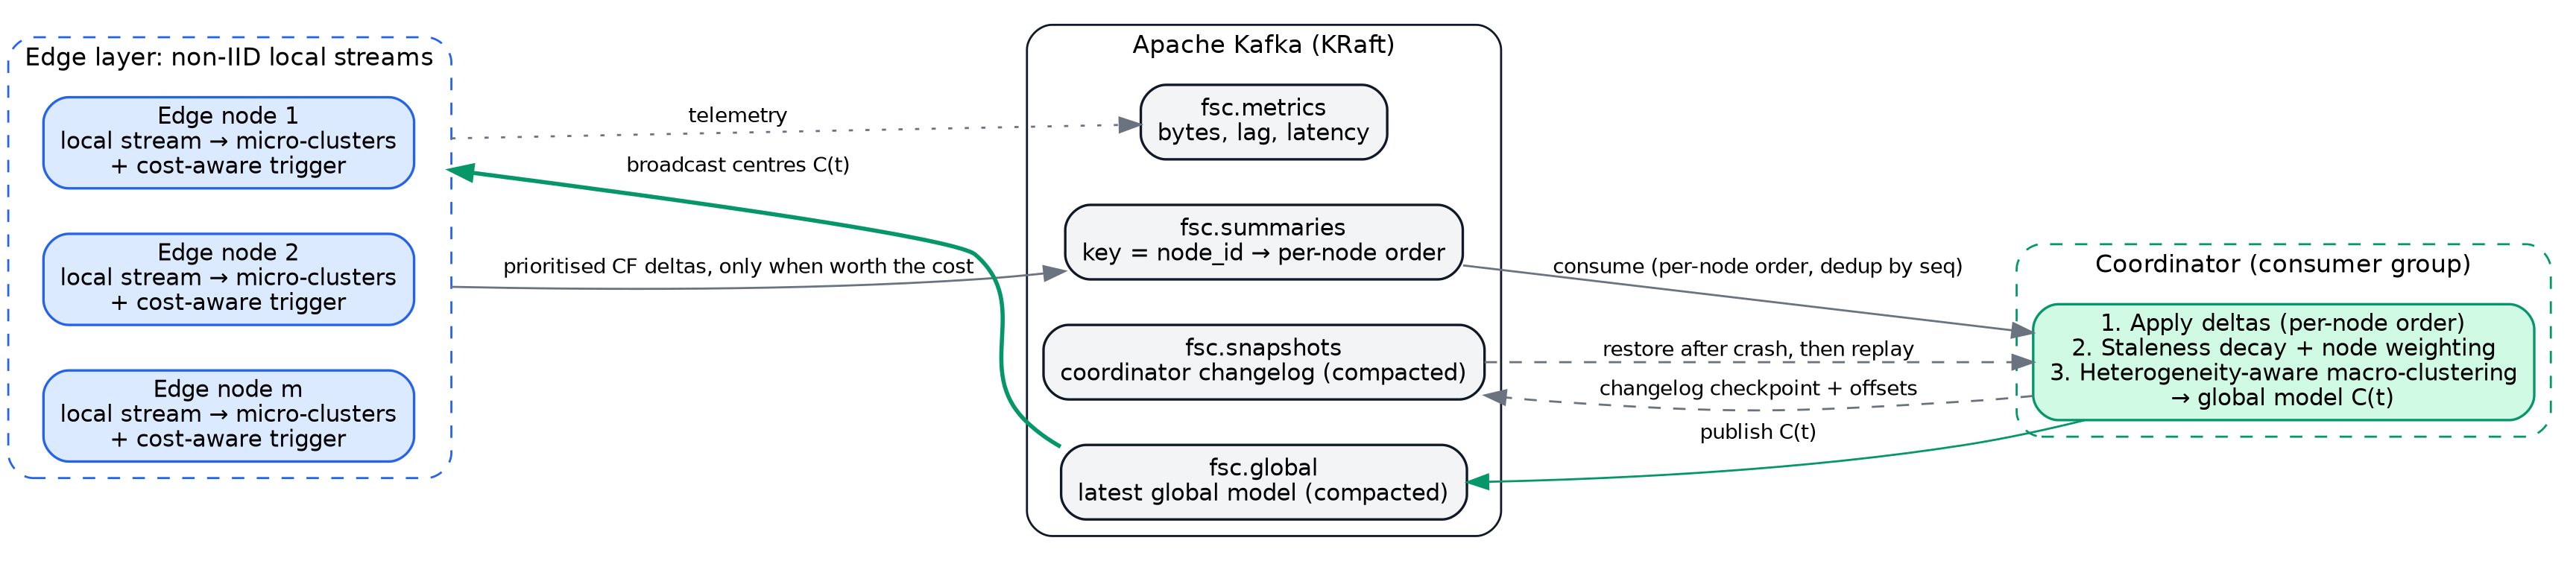
\includegraphics[width=0.92\textwidth]{../docs/figures/architecture.png}
\caption{FedCAST over Apache Kafka. Edge nodes publish prioritised CF deltas only when they are worth their byte cost. The coordinator applies them in per-node order, checkpoints its state to a compacted changelog, and broadcasts the global model on a compacted topic that the edges use to compute staleness.}\label{fig:arch}
\end{figure*}

Kafka~\cite{kreps2011kafka,wang2015kafkareplication} is not only the transport in FedCAST. Four of its semantics are part of the algorithm's correctness argument (Table~\ref{tab:kafka}).

\begin{table}[t]
\centering\small
\caption{Kafka semantics used by FedCAST.}\label{tab:kafka}
\begin{tabular}{@{}p{0.34\columnwidth}p{0.58\columnwidth}@{}}
\toprule
Semantics & Role in FedCAST\\
\midrule
Per-partition order, key $=$ node & Deltas of a node are applied in the order produced; a delta may assume its predecessor.\\
Idempotent producer + per-node sequence numbers & Retries on lossy links never double-apply a delta; replays after a crash are ignored.\\
Replayable log + committed offsets & A restarted coordinator replays only what it had not yet checkpointed; nodes never resend.\\
Log compaction & \texttt{fsc.snapshots} is a changelog holding one record per node (the server-side CFs and the offsets they reflect); \texttt{fsc.global} always holds the latest model, also for late joiners.\\
\bottomrule
\end{tabular}
\end{table}

\paragraph{Topics} \texttt{fsc.summaries} (8 partitions, key \texttt{node-}$i$) carries deltas. \texttt{fsc.snapshots} (compacted) is the coordinator's changelog. \texttt{fsc.global} (compacted, one partition) carries the model. \texttt{fsc.raw} is used only by the centralised baseline, and \texttt{fsc.metrics} carries telemetry.

\paragraph{Wire format} Messages use a fixed little-endian binary layout: a 20-byte header (kind, node, sequence number, time, counts, dimension) followed by packed arrays. The size of a pending delta is therefore known \emph{before} encoding, which the trigger~\eqref{eq:trigger} requires, and decoding is zero-copy. JSON would be 3--5$\times$ larger and of variable size. Avro or Protobuf would require a schema registry service.

\paragraph{Exactly-once state and recovery} The coordinator follows the state-store-plus-changelog pattern of stream processors~\cite{carbone2017flinkstate}. Every few seconds it writes, per node, a full CF record to \texttt{fsc.snapshots}, with the last applied sequence number and the \texttt{fsc.summaries} offsets as record headers, and then commits the offsets. On restart it reads the compacted changelog, restores all node states, and resumes \texttt{fsc.summaries} at the checkpointed offsets. Records after the checkpoint are applied again, and any record at or below a node's restored sequence number is ignored. The recovered state is therefore identical to that of an uninterrupted coordinator (Section~\ref{sec:rq4}).

\paragraph{Low-memory deployment} The broker runs in KRaft mode (no ZooKeeper) with a 256\,MB heap. We measured 317\,MB idle and 423\,MB peak RSS under a 300k-message load test; in Docker with a 512\,MB cap it never ran out of memory. All simulated nodes share one Python process ($\approx$150\,MB) with one idempotent producer each, and the coordinator needs $\approx$140\,MB. The complete system runs in under 1\,GB of RAM, which makes it reproducible on commodity laptops without Flink or Spark.

\paragraph{Two execution modes, one code base} The same \texttt{EdgeNode}, policy, codec and coordinator classes run (i) against a real broker and (ii) inside a deterministic discrete-event simulator. The simulator replaces the broker with seeded per-node links (delay, jitter, bandwidth cap, loss with retransmission, outages) that preserve per-key FIFO order and count retransmitted bytes. The simulator enables thousands of seeded runs. The Kafka mode provides the systems measurements and validates the simulator's byte accounting against Kafka's producer statistics.
